\documentclass{article}
\usepackage[utf8]{inputenc}
\usepackage{graphicx,fancyhdr,amsmath,amssymb,amsthm,subfig,url,hyperref,enumerate}

% For payoff matrices
\usepackage{multirow,enumerate,array,float}
\usepackage[margin=1in]{geometry}

% For figures
\usepackage{graphicx}
\graphicspath{ {./figures/} }

\begin{document}
\title{Improving healthcare outcomes and cost through analysis and design of provider incentives}
\author{Keyan Pishdadian\\University of Washington\\\texttt{keyanp@cs.washington.edu}}
\date{March 2020}

\maketitle

\begin{abstract}
Provider decision making plays a critical role in patient outcomes and national healthcare spending. Creating robust incentive structures to underlie provider decision making are vital to ensuring the delivery of high quality care and adequately managed costs. Despite their importance these incentive structures are poorly designed both financially and from a provider risk perspective. In this paper I analyze the inefficiencies and sub-optimal equilibria that result from the use of classic incentive systems, then extend recent ideas to propose a hybrid incentive structure that increases provider profits, improves patient outcomes, and reduces wasteful spending.
\end{abstract}

\section{Introduction}
Healthcare is a socially and economically important aspect of the modern United States. Roughly 1/6th of US consumer spending \cite{econharvard} and ${\sim}48$\% of federal spending \cite{federalspend} goes towards some form of healthcare. The success, efficiency, and outcomes of this market reflect directly on the viability and happiness of American citizens and the US economy. The decision making of physicians plays a integral role in this system, with roughly 80\% of all expenditure being a result of physicians' decisions \cite{trust}. One becomes concerned with this control when comparing US healthcare expenditure to other developed countries \cite{econharvard}, just why is expenditure so much higher in the US without better outcomes \cite{acoecon}?

At the root of the issue is that the healthcare market is unlike other normal markets where there is a buyer and a seller, with the buyer fully knowing what it is they want and having transparency into the price being offered by the seller \cite{msdt}. Rather, in this market there are many agents interacting directly or indirectly within a single healthcare transaction. This results in a complex web of interdependencies between the agents (Fig. \ref{fig:agentdep}) which significantly complicates construction of effective incentive structures. Additionally the patient has little control in their outcomes aside from selecting a provider. In fact, the patient-provider relationship is a clear example of a \emph{principle-agent problem} \cite{principle} where the provider (the ``agent") must make diagnosis and care decisions that impact the patient (the ``principle"), but the provider/agent is motivated to act in their own best interests and not in the best interest of the patient/principle \cite{msdt} (Fig. \ref{fig:overtreat}). Simultaneously, the provider is engaged in a game with other providers that closely resembles a ``prisoner's dilemmas"\footnote{For a thorough treatment of the prisoner's dilemma, refer to any number of game theory texts, e.g. \cite{networks}}, ultimately the decision making of any one provider has externalities on the health of the entire patient population, with a future decrease in overall health leading to an increase in the required volume of care to sustain proper health \cite{blended}.

In this paper I present each of the prevailing provider incentive structures, examine their benefits and inefficiencies, then use an adapted simplified model to formalize the resulting equilibria reached in each system. I then extend recent ideas from Accountable Care Organizations (ACOs) to propose and analyze a hybrid incentive structure that increases provider profits and improves patient outcomes primarily through the introduction of a \emph{trust score}.

\begin{figure}[H]
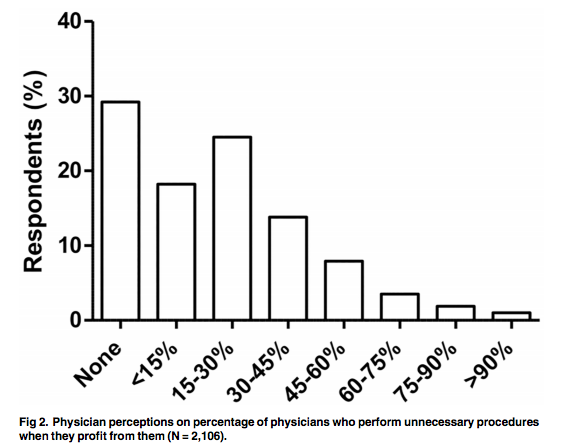
\includegraphics[height=7cm]{overtreat}
\centering
\caption{Provider responses when surveyed and asked what percentage of other physicians they think perform unneeded procedures financial gain \cite{overtreat}. Even other providers do not believe that healthcare professionals are acting in the best interests of patients.}
\label{fig:overtreat}
\end{figure}

\section{Setup}

\subsection{Agents}
To begin analysis of the current state of healthcare it is required to examine who is involved and what they are optimizing for. Because the scope of this system is large, I limit the number of agents and make some assumptions about their motivations to simplify the future model. An overview of the agents is provided in Fig. \ref{fig:agentdep}, and they are summarized below.

\paragraph{Payer:}The payer can be thought of as both an individual patient or alternatively some entity which is responsible for paying for services rendered to others. Generally the latter case would be an employer or government which is providing health insurance to others at cost. While insurance companies are also considered a payer, their interests are outside the scope of this work. Note that oftentimes there are multiple payers involved in a single healthcare transaction, although here it is assumed that they are all aligned with respect to their goals.

Ultimately the payer seeks to minimize cost, while maximizing quality of service. In the case of a patient the desire to maximize quality of service is self-explanatory, and in the case of an employer/government the intention is that high quality of service will mean higher general health and less future demand for healthcare, which drives down cost.

\paragraph{Provider:}These are any individuals rendering services for payers. Generally providers can be thought of as physicians. Providers seek to maximize revenue\footnote{In order to simplify the model I ignore any altruistic behavior and moral incentives that I imagine (and hope) are present to some extent.} to themselves and also minimizing financial and professional risk (e.g. malpractice lawsuits).

The provider is the central agent in this model because as mentioned previously, their decisions account for ${\sim}80$\% of healthcare spending \cite{trust}. Importantly the payoff of any one provider is influenced by the collective behavior of other providers in the system. A provider may choose to render low quality service and thus negatively affect the health of a patient and through this they can impart externalities on other providers, whether those are negative or positive depends on the payment system.

\paragraph{Hospital:}A hospital manages the compensation of providers and negotiates with payers to determine costs. Hospitals seek to maximize revenue by minimizing cost. Traditionally this also means maximizing volume of services rendered while minimizing quality of those services, but this fact can vary with the compensation structure being used. This paper does not focus on the actions of a hospital other than presenting them as a possible organizer and controller of providers given that the hospital is designing the provider compensation system.

\begin{figure}[H]
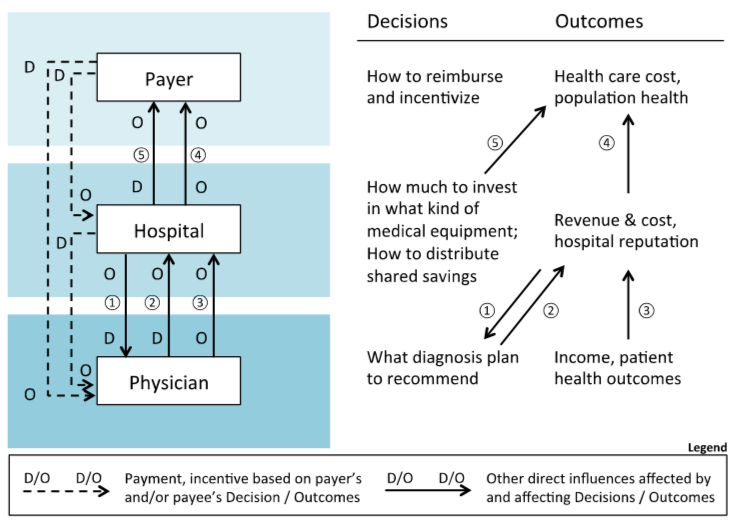
\includegraphics[height=7cm]{agentdep}
\centering
\caption{Agent interdependence diagram which shows the complex network of interactions between payers, providers (Physician), and hospitals. In this work I focus on controlling the provider decision making process (relations $1$ and $2$) as a means of improving payer health outcomes and cost (relation $4$) \cite{msdt}.}
\label{fig:agentdep}
\end{figure}

\subsection{Incentive Modeling} \label{sec:modeling}
In order to create a framework to analyze provider actions and payoffs in the existing and proposed payment models, the following set of notation is introduced (adapted from \cite{trust}\cite{blended}) to represent the different variables involved:

\begin{itemize}
    \item \textbf{V} - Volume of services. An independent variable that is decided on by the provider.
    \item \textbf{Q} - Quality of services. An independent variable that is a result of provider decisions.
    \item \textbf{E} - Externalities on other providers. Dependent on the payment model and provider quality decisions.
    \item \textbf{C} - Capitation rate (explained in Section \ref{sec:capitation}). Dependent on the payment model.
    \item \textbf{B} - Bonus incentive. Dependent on the payment model and provider decisions.
    \item \textbf{T} - Trust score. Dependent on provider decisions.
\end{itemize}

In this model the provider is able to control $V$ and $Q$, by either performing a low or high volume of service ($V_{low}$, $V_{high}$), and either low or high quality service ($Q_{low}$, $Q_{high}$), the pair of provider actions in a model is represented as $(V, Q)$.

Externalities are unique in that they are applied to \emph{other} providers but determined by an individual provider quality decision. The notation $E_{Q_{high}}$ and $E_{Q_{low}}$ are used to represent the resulting externalities caused by a decision to give high and low quality service, respectively. In some payment models $E_{Q_{high}} > E_{Q_{low}}$, while in others $E_{Q_{high}} < E_{Q_{low}}$, but one can imagine that an ideal system is one that incentivizes providing high quality service by ensuring that results in positive externalities on other providers.

Capitation rate is an element specific to the \textbf{capitation} payment model as explained in Section \ref{sec:capitation}. For the purposes of explaining this variable it can be said that its magnitude is determined by the provider choice of quality where higher quality service results in a higher capitation rate. Using similar notation as for externalities it is always the case that $C_{Q_{high}} > C_{Q_{low}}$.

The \emph{bonus incentive} ($B$) and \emph{trust score} ($T$) variables are new concepts that I leverage to sway provider decision making by rewarding desirable provider behavior. The bonus is adapted from ideas presented in ACOs (see Section \ref{sec:aco}), this value is computed based on reaching certain benchmarks over a defined interval. The trust score is a form of a reputation system \cite{tim} that uses patient outcome surveys and peer-provider ratings to assess provider behavior, this score is used to apply an additional bonus to a provider for responsible actions they have taken in this and previous periods of time.

\section{Existing Payment Models}
In this section I review the two major incentive structures used for provider payment, \textbf{fee-for-service} and \textbf{capitation}. Discussion of the issues with each structure gives motivation to understanding the novel payment structure used by ACOs.

\subsection{Fee-for-service}
This model is most familiar to anyone who has interfaced with US healthcare. Here a provider is payed for each service rendered (e.g. surgery, office visit). Hence the payment to the provider is a direct linearly increasing function of the volume of services provided. Of course a clear conflict of interest is presented, providers are incentivized to provide a high volume of high cost services, regardless of need and thus with low quality. Aside from ethical considerations, the outcome of the patient has no bearing on the payoff of the provider. This observation is not surprising given the principle-agent backdrop coloring this relationship, and it has been documented that patients and other providers have formed an expectation that some providers optimize decisions on financial reward (Fig. \ref{fig:overtreat}) \cite{econharvard}\cite{overtreat}.

So what does this method get right? That same indifference to cost that begets high volume service may also allows access to expensive services that may give good results but have low probability of success. When providers do not fear increased spending then they are free to explore new treatment methods, equipment, medications, and procedures.

Using the incentive model the payoff under this payment system as is represented as:
\begin{equation} \label{eq:ffs}
    \text{payoff} = V + Q + E
\end{equation}

One can assume that any provider will choose to provide a high volume of service as it is directly increases earnings, but how does this model affect quality decisions? By choosing to offer high quality service, a provider actually imparts \emph{negative} externalities for other providers, who would now have fewer patients to treat and thus less service volume to bill for, therefore $E_{Q_{low}} > E_{Q_{high}}$. It follows that to maximize payoff according to Equation \ref{eq:ffs} the best response of any provider to other providers in the system is to always choose $(V_{high}, Q_{low})$, an unfortunate outcome for patients and supporting payers who must foot the bill. When considering only providers in the system, this action is the unique Nash equilibrium \cite{blended} and is Pareto optimal for all providers.

\subsection{Capitation} \label{sec:capitation}
The capitation model is on the other end of the spectrum relative to fee-for-service models. Here a provider is paid a fixed sum, the \emph{capitation rate}, for an agreed upon length of time for each patient that they oversee the health of. There are a wide range of methods used to compute capitation fees and payments structures that are outside the scope of this paper and discussed elsewhere, e.g. \cite{capfees}. Overall the principle is that providers want to reduce the number of services rendered and keep patients healthy so that they do not exceed the negotiated rate of payment per patient. Because any amount of spending beyond the negotiated capitation rate is entirely the responsibility of the provider/hospital, this model shifts significant risk to the provider to keep costs low, but has potential for greater financial payoff if the total cost of services rendered is significantly below the capitation fee.

Supporters of this model cite that it succeeds in reducing provider incentives to provide high volume services that are driven more by billing ability than by patient need \cite{blended}. However, there is fear that this design results instead in a low volume of low quality services because the capitation rate calculation penalizes high expenditure and rewards higher quantities of treated patients. Let us explore these theories.

Using the incentive model the payoff under this payment system as is represented as:
\begin{equation} \label{eq:cap}
    \text{payoff} = V + Q + E + C
\end{equation}

Because the volume of services provided is inversely correlated with earnings, providers are incentivized to minimize volume and always play $V_{low}$. Uniquely, the decision of what level of quality to provide is less clear. By choosing to provide high quality services there is an increase of collective patient health which causes \emph{positive} externalities for other providers, who would now have fewer/healthier patients to treat and thus reduce their future costs, therefore $E_{Q_{low}} < E_{Q_{high}}$. For similar reasons, as mentioned in Section \ref{sec:modeling}, the capitation rate is positively correlated with quality of service rendered, $C_{Q_{high}} > C_{Q_{low}}$. But simultaneously high quality service means more time and cost from the provider so $Q_{low} > Q_{high}$. If simple values are set for the model parameters an interesting problem arises as demonstrated in Table \ref{table:cap}.

\begin{table}[H]
\centering
  \setlength{\extrarowheight}{2pt}
  \begin{tabular}{*{4}{c|}}
    \multicolumn{2}{c}{} & \multicolumn{2}{c}{Other Providers (O)}\\\cline{3-4}
    \multicolumn{1}{c}{} &  & $(V_{low}, Q_{low})$  & $(V_{low}, Q_{high})$ \\\cline{2-4}
    \multirow{4}*{Provider (P)} &
      $(V_{low}, Q_{low})$
        & $\text{(P) } 2 = 0+0-1+3$ & $\text{(P) } 4 = 0+0+1+3$ \\ $$
        & $$
        & $\text{(O) } 2 = 0+0-1+3$ & $\text{(O) } 1 = 0-3-1+5$ \\\cline{2-4} &
      $(V_{low}, Q_{high})$
        & $\text{(P) } 1 = 0-3-1+5$ & $\text{(P) } 3 = 0-3+1+5$ \\ $$
        & $$
        & $\text{(O) } 4 = 0+0+1+3$ & $\text{(O) } 3 = 0-3+1+5$ \\\cline{2-4}
  \end{tabular}
  \caption{Payoff matrix showing outcomes for the main provider (P) and other providers in the network (O). Assume that all providers play $V_{low}$ which is set to simply $0$, and that the other parameters are set to: $Q_{low} = 0, Q_{high} = -3, E_{Q_{low}} = -1, E_{Q_{high}} = 1, C_{Q_{low}} = 3, C_{Q_{high}} = 5$. Recall that the quality action of one provider affects their own capitation rate, but affects the externality value of the \emph{opposite} provider. Payoffs are calculated using Equation \ref{eq:cap}. A prisoner's dilemma is present, with providers reaching a unique Nash equilibrium of both playing $(V_{low}, Q_{low})$.}
\label{table:cap}
\end{table}

In this model a prisoner's dilemma arises between providers. Notice that if any provider plays $(V_{low}, Q_{high})$ while another plays $(V_{low}, Q_{low})$, the former is incentivized to change their response to $(V_{low}, Q_{low})$ to increase their payoff slightly. If both providers play $(V_{low}, Q_{high})$ then there is incentive to switch to $(V_{low}, Q_{low})$ for a slightly higher payoff as well. In fact there is a non-Pareto optimal unique pure Nash equilibria of $(V_{low}, Q_{low}), (V_{low}, Q_{low})$ giving payoff $(2, 2)$. Meanwhile if all providers acted cooperatively and played $(V_{low}, Q_{high})$ they could reach a Pareto optimal outcome with the higher payoff $(3,3)$, increasing their own earnings and improving outcomes for patients.

Collectively all providers are better off if the health of the patient population in aggregate is good, as this means those patients will impose lower costs on each provider, but each provider's \emph{best response} strategy when making a care decision is ultimately to still provide low volume low quality care and free-ride on any provider that might be providing high volume high quality care.

\subsection{Accountable Care Organizations (ACOs)} \label{sec:aco}
ACOs were introduced as an attempt to mitigate some of the issues with both of the aforementioned payment structures. Formally enacted as part of the Patient Protection and Affordable Care Act of 2010 (``Obamacare"), over 10.5 million Medicare patients have been assigned to ACOs over recent years and there are data to support that there has been significant federal savings using the system \cite{acos}.

An ACO is a group of providers who choose to join that organization and together treat Medicare patients. The Centers for Medicare \& Medicare (CMS) is a federal agency which sets a maximum expenditure benchmark for that ACO based on prior Medicare expenses and cost forecasting. Together providers in the ACO render services using a standard fee-for-service payment model, but if the total spending during a pre-defined time interval is below the expenditure benchmark then the ACO receives up to ${\sim}50$\% of the savings as a cash incentive bonus, depending on an additional \emph{quality score} \cite{acos}. The exact computation of earnings depends on the negotiated ACO incentive structure and the quality score which is determined by evaluating performance on annually set CMS benchmarks, e.g. percentage of patients provided with preventative screening and influenza vaccination (detailed quality benchmarks can be found on the CMS website \cite{cms}). Accordingly a representative formula for savings bonus calculation would be (adapted from \cite{acos}):

\begin{equation}
    B = \max (0, 0.5 * (\text{Spending Benchmark} - \text{Actual Spending}) * \text{Quality Score})
\end{equation}

This incentive structure has some nice intuitive properties. The spending benchmark and associated savings bonus escape incentives to overspend with high volume seen in the fee-for-service model, while the use of a quality score avoids the natural best response of underspending through low quality observed in the capitation model. Together with the quality score, these properties work together to align the incentives of the payer/patient with that of the provider \cite{acoecon}. The inter-provider relationship is also improved (within an ACO) because the spending and quality benchmarks are computed for collective metrics of all providers in the organization.

Using the incentive model the payoff under this payment system as is represented as:
\begin{equation}
    \text{payoff} = V + Q + E + B
\end{equation}

At first ACOs seem to solve all our issues, but they introduce their own problems. Namely,
\begin{itemize}
    \item \textbf{Centralization} - The ACO system relies on a federal central authority (CMS) to act as an altruistic dictator that controls benchmark setting, quality rankings, and provides financial incentives using the federal budget. It is not clear how this system could work without such an authority.
    \item \textbf{Concentration of power} - ACOs are groups of sometimes many thousands of physicians, often resulting in multiple hospitals grouping together to form a single ACO \cite{acoethics}. This leads itself to a relatively small number of large groups concentrating power and having increased healthcare market share. With this size comes the ability to control the market and raise prices for payers through aggressive negotiation with insurance companies. This may even entirely offset any expected savings for the payer \cite{acoecon}.
    \item \textbf{Coordination of care} - Patients often require attaining care from providers outside of the patient's main ACO, generally through referrals. This introduces significant complexity because those providers are not as invested in the long term health of those patients because those patients do not factor into the quality score for the referred-from-ACO \cite{acoecon}.
    \item \textbf{Bonus sharing} - The hospitals organizing the ACO control the savings bonus and how to allocate it amongst providers. Determining an optimal distribution method is complicated and prone to hospitals acting in their own self-interest \cite{inflation}. Additionally there is no aspect of the design that rewards good actors and penalizes bad actors. ACOs are left to their own decisions on how to appropriately compensate providers that have positive externalities on the system, and how to even determine those externalities.
\end{itemize}

\section{Hybrid Approach} \label{sec:reqs}
Given the broad overview of prevailing payment models, how could a better system be implemented? Here I propose a new system modeled to meet the following requirements:

\begin{itemize}
    \item \textbf{Incentive alignment} - The interests of payers and providers should be aligned, escaping the principle-agent problem of misaligned incentives present in the fee-for-service and capitation systems.
    \item \textbf{Positive externalities} - The provider decision equilibrium should shift to low volume and high quality services. As this decreases costs on the collective system and also improves patient outcomes, reducing future demand on other providers.
    \item \textbf{(Partial) Decentralization} - There should be no central authority which pays financial rewards because such a system could not scale to cover the largely private US healthcare system. Additionally, concentration of power into a small number of large networks should be avoided to prevent potential adverse market impacts.
    \item \textbf{Reputation influenced rewards} - Good behavior bonuses should be paid out based on individual provider behavior, not the collective behavior of a large group of providers. This avoids the complexity of designing bonus sharing systems organized by a hospital, and also escapes the problems with coordination of care associated with network oriented benchmarking in ACOs.
\end{itemize}

\subsection{Provider Trust Network Model} \label{sec:ptnm}
I propose a hybrid system borrowing ideas from several existing methods, called the \textbf{Provider Trust Network Model}. Under the proposed model there is a federally funded central authority (denoted the \emph{trust agency}) that maintains an objective provider-specific reputation score, computed using quality metrics similar to those used by an ACO, long term patient outcome surveys, and peer reviews completed by fellow providers. This is the provider \emph{trust score} $T$, and is used to modulate provider payments. Computation of the trust score is discussed in more detail in Section \ref{sec:trustscore}.

The trust agency also sets spending benchmarks per provider specialty, based on cost forecasting and nationwide historical data. The spending benchmarks are shared with insurance companies who individually assess bonus scores for each provider based on how much that provided billed that specific insurance company during the specified time window. This means each provider receives a distinct bonus from each insurance provider they accept, which is mostly a side effect of the fragmented US healthcare system but provides the advantage of decentralization of power over bonuses from large groups to the providers themselves.

The main aspects of payment computation done by the hospital are based on a blended model of low magnitude capitation rates for routine services and a standard fee-for-service component for more complex and non-standard procedures \cite{blended}. This approach eliminates provider risk that can occur in a pure capitation model where providers may give low quality services in an effort to reduce costs. Although this may seem to encourage higher spending and billing for procedures that would qualify as non-standard and eligible for fee-for-service, I propose this is controlled for by the provider trust score.

Therefore provider payoffs in the model, for each period, are represented as:
\begin{equation} \label{eq:ptnm}
    \text{payoff} = \min(V + C + B, (V + C + B) * T) + E + Q
\end{equation}

\subsection{Trust Score} \label{sec:trustscore}
Trust scores are computed using a discounted reputation value. Each provider has a single \textbf{trust ranking} $t$ which is running total of their ``trust". Let $i$ be some pre-defined time period of service, e.g. a financial quarter, the trust ranking for a provider for a single time period is defined as $t_i$. In any period the provider may take actions that increase or decrease their trust ranking for that period and sum to the final value $t_i$. Therefore the trust ranking for any period $i$ is defined as:
\begin{equation}
    t_i = t_{i - 1} + \Delta t_i
\end{equation}

The change in trust ranking for any single round is determined by the provider decisions during that round, as reported through quality metrics and patient outcomes surveys. If these mechanisms are properly designed then desirable behavior should increase the trust ranking, while undesirable/uncooperative behavior decreases it. As such it is expected that for any period, $Q_{high} \Rightarrow +\Delta t$, $Q_{low} \Rightarrow -\Delta t$, and $V_{high} \Rightarrow -\Delta t$.

The \textbf{trust score} $T$ for the current period $k$ is defined as a summation across all of that providers trust rankings for every period $1 \dots k$ and scaled such that earlier time periods are exponentially discounted. The final trust score is based on how close the providers discounted trust ranking sum is to the maximum possible trust ranking $t_{max}$ (assuming perfect behavior for every round up to $k$), multiplied by a scale factor $\chi$. The scale factor $\chi$ can be thought of the percentage of $t_{max}$ that a provider must have in order to be considered full trustworthy. This produces a value $T$ for the current round that is in the interval $[0, 1]$. The full formula is as follows:

\begin{equation}
    T = \min \left( 1, \frac{\sum_{i=1}^k t_i^{i / k}} {t_{max} * \chi} \right)
\end{equation}

Exponential discounting allows for scaling the provider payment based on current and past period behavior, while also allowing some flexibility in the cutoff for maximum trust payout through the use of $\chi$. This avoids undesirable provider behavior in one period that was done for a large and inappropriate fee-for-service payoff, only to later have poor patient surveys and missed quality benchmarks.

\subsection{Analysis}
Due to the difficulty in performing the discounted trust score computations by hand, a small simulation program was written to validate this model under each possible play tactic. It is included in the submission and can be executed by running: \texttt{\$ python3 provider\char`_trust\char`_network.py}.

It can be shown, after making some assumptions for the payoff variables in line with the design of this model, that the Provider Trust Network Model can successfully push providers into an equilibrium that achieves this systems requirements. Results from analysis via simulation are provided in Table \ref{table:ptnlow} and Table \ref{table:ptnhigh}. Fulfillment of those requirements outlined in Section \ref{sec:reqs} is justified below:

\begin{itemize}
    \item \textbf{Incentive alignment} - The equilibrium created makes $(V_{low}, Q_{high})$ the unique pure Nash equilibrium and a Pareto optimal outcome for all providers (Table \ref{table:ptnlow}), ensuring low cost and high quality services are provided to patients.
    \item \textbf{Positive externalities} - Giving high quality services to patients causes positive externalities for other providers by improving overall population health.
    \item \textbf{(Partial) Decentralization} - This requirement is discussed in designing of the trust agency and benchmarks in Section \ref{sec:ptnm}.
    \item \textbf{Reputation influenced rewards} - Past bad behavior strongly influences outcomes with undesirable actions resulting in extreme low payoff. It should be noted that this model results in negative payoffs, which would likely be impossible to implement in reality.
\end{itemize}

\begin{table}[H]
\centering
  \setlength{\extrarowheight}{2pt}
  \begin{tabular}{*{4}{c|}}
    \multicolumn{2}{c}{} & \multicolumn{2}{c}{Other Providers (O)}\\\cline{3-4}
    \multicolumn{1}{c}{} &  & $(V_{low}, Q_{low})$  & $(V_{low}, Q_{high})$ \\\cline{2-4}
    \multirow{2}*{Provider (P)}  & $(V_{low}, Q_{low})$ & $(-29, -29)$ & $(-29, 9)$ \\\cline{2-4}
    & $(V_{low}, Q_{high})$ & $(9, -29)$ & $(9, 9)$ \\\cline{2-4}
  \end{tabular}
\caption{Payoff matrix showing outcomes for the main provider (P) and other providers in the network (O) after the fourth period using the Provider Trust Network Model. The score for the row player is listed first. Assume that all providers play $V_{low}$ which is set to simply $0$, and that the other parameters are set to: $Q_{low} = 2, Q_{high} = 4, E_{Q_{low}} = -1, E_{Q_{high}} = 1, C_{Q_{low}} = 1, C_{Q_{high}} = 3$. Trust rankings are adjusted per period by applying these change values based on the provider actions: $Q_{low} \Rightarrow -\Delta 2$, $Q_{high} \Rightarrow +\Delta 2$, $V_{low} \Rightarrow \Delta 0$, $V_{high} \Rightarrow -\Delta 2$. Payoffs are calculated using Equation \ref{eq:ptnm}. There is a unique pure Nash equilibrium outcome when both providers play $(V_{low}, Q_{high})$, it is also a Pareto optimal outcome.}
\label{table:ptnlow}
\end{table}

\begin{table}[H]
\centering
  \setlength{\extrarowheight}{2pt}
  \begin{tabular}{*{4}{c|}}
    \multicolumn{2}{c}{} & \multicolumn{2}{c}{Other Providers (O)}\\\cline{3-4}
    \multicolumn{1}{c}{} &  & $(V_{high}, Q_{low})$  & $(V_{high}, Q_{high})$ \\\cline{2-4}
    \multirow{2}*{Provider (P)}  & $(V_{high}, Q_{low})$ & $(-93, -93)$ & $(-93, 3)$ \\\cline{2-4}
    & $(V_{high}, Q_{high})$ & $(3, -93)$ & $(3, 3)$ \\\cline{2-4}
  \end{tabular}
    \caption{Payoff matrix showing outcomes for the main provider (P) and other providers in the network (O) after the fourth period using the Provider Trust Network Model. The score for the row player is listed first. Assume that all providers play $V_{high}$ which is set to a large payoff of $5$ to represent this models fee-for-service component, and that the other parameters and trust ranking change values are equal to their values in \ref{table:ptnlow}. There is a unique pure Nash equilibrium outcome when both providers play $(V_{high}, Q_{high})$, it is also a Pareto optimal outcome (assuming Volume cannot be changed). However the payoff is lower than if providers choose $V_{low}$ as in \ref{table:ptnlow}.}
\label{table:ptnhigh}
\end{table}

\section{Conclusions}
In this work I reviewed recent literature on provider payment systems and discussed some of the advantages of each system. Through this review I have given motivation to the presentation of a novel approach to designing compensation systems that leverages a trust agency and decentralized benchmark scoring in order to create the \textbf{Provider Trust Network Model}, which is a reputation influenced payment scheme. While this system has theoretical benefits over traditional fee-for-service, capitation, and modern ACOs, further research is needed to assess if these benefits can be realized in the US healthcare market.

The primary risks with potential implementation would be the logistics and design of the trust agency, trust score, and per-provider quality benchmarks. Could the trust agency feasibly manage the complexity of tracking and storing trust scores for all US providers across many years? What risks are introduced by centralization of the trust agency? How can safeguards be designed to prevent adversarial attacks on the trust agency? Additionally, there are concerns with hospitals and providers being able to supply the necessary data to compute these scores and benchmarks, a task that has already proven to be difficult for ACOs \cite{acoecon}.

Modeling incentives in a complex and multi-agent environment is challenging and imprecise. Developing frameworks such as this is a useful tool for identifying potential directions for further investigation or provide theoretical validation for ideas prior to attempting implementation. It is impossible to fully model all interactions within the healthcare system, but analyzing provider payment schemes shows that even simple modeling can uncover areas for improvement. I hope that future researchers in this area will invest effort into exploring the benefits and feasibility of reputation driven systems to more precisely modulate provider behavior and improve patient outcomes.


%--------------------------------- Bibliography ----------------------------------

\clearpage

\begin{thebibliography}{8}

\bibitem{federalspend}
The True Cost of Health Care: An Analysis of Americans’ Total Health Care Spend. https://bit.ly/39wbFzi

\bibitem{econharvard}
Mankiw NG. (2017) The Economics of Healthcare.

%6
\bibitem{trust}
Djulbegovic, Benjamin \& Hozo, Iztok \& Ioannidis, John. (2014). Modern health care as a game theory problem. European Journal of Clinical Investigation. 45. 10.1111/eci.12380

\bibitem{overtreat}
Lyu H, Xu T, Brotman D, Mayer-Blackwell B, Cooper M, Daniel M, et al. (2017). Overtreatment in the United States. PLoS ONE 12(9): e0181970. https://doi.org/10.1371/journal.pone.0181970

%4
\bibitem{blended}
DeVoe, J. E., \& Stenger, R. (2013). Aligning provider incentives to improve primary healthcare delivery in the United States. OA family medicine, 1(1), 7. doi:10.13172/2052-8922-1-1-958

%5
\bibitem{msdt}
Zhang, H., Wernz, C. \& Slonim, A.D. (2016). Aligning incentives in health care: a multiscale decision theory approach. EURO J Decis Process 4, 219–244. https://doi.org/10.1007/s40070-015-0051-3

\bibitem{principle}
Eisenhardt, K. (1989). Agency Theory: An Assessment and Review. The Academy of Management Review, 14(1), 57-74. www.jstor.org/stable/258191

\bibitem{networks}
David, E., Kleinberg, J. (2010). Networks, Crowds, and Markets: Reasoning About a Highly Connected World. Cambridge University Press, USA. https://www.cs.cornell.edu/home/kleinber/networks-book/

\bibitem{acos}
Redding, K. (2018). Participation and Performance in Accountable Care Organizations, Doctoral Dissertation.

\bibitem{capfees}
Iezzoni, Lisa I. et al. (1998). Paying More Fairly for Medicare Capitated Care. New England Journal of Medicine. https://doi.org/10.1056/NEJM199812243392613

\bibitem{acoecon}
Blackstone, E. A., \& Fuhr, J. P., Jr (2016). The Economics of Medicare Accountable Care Organizations. American health \& drug benefits, 9(1), 11–19.

\bibitem{cms}
https://www.cms.gov/Medicare/Medicare-Fee-for-Service-Payment/sharedsavingsprogram/Downloads\-/2018-and-2019-quality-benchmarks-guidance.pdf

% 1
% Cite as complicated approach by modifying how hospitals bill for services
\bibitem{inflation}
Agee, M.D., Gates, Z. (2013). Lessons from Game Theory about Healthcare System Price Inflation. Appl Health Econ Health Policy 11, 45–51. https://doi.org/10.1007/s40258-012-0003-z

\bibitem{acoethics}
Virtual Mentor. 2013;15(2):156-161. doi: 10.1001/virtualmentor.2013.15.2.pfor1-1302.

\bibitem{tim}
Roughgarden, T. (2016). Asymmetric Information and Reputation Systems. http://timroughgarden.org/f16/l/l12.pdf

\end{thebibliography}

%-------------------------------------------------------------------

\end{document}
